
\documentclass[fleqn]{article}     


% -------------------------------------------------- %
% ---------------- Import Packages ----------------- %
% -------------------------------------------------- % 




% ----------------- Font Settings ------------------ %

    % allow special charcters (ä, ö, ü, ...)
\RequirePackage[utf8]{inputenc}
    % help with special charcters (ä, ö, ü, ...)
\RequirePackage[T1]{fontenc}   
    % Auto Translation (eg.: "figure" --> "Abbildung")
\RequirePackage[ngerman]{babel}           
    % Text Font Style = Times New Roman
\RequirePackage{newtxtext}
    % Math Font Style = Times New Roman
\RequirePackage{newtxmath}                 




% ----------------- Mathematics ------------------ %

    % general mathematics
\RequirePackage{mathtools} 
    % physics unit notation
\RequirePackage{siunitx}   
\sisetup{
  per-mode=symbol,
  separate-uncertainty=true,
  round-mode=places,
  round-precision=2,
  locale = DE
}      



% ------------ Citation & Reference -------------- %

    % hyper-reference within document
\RequirePackage{hyperref}    
    % fix hyper-reference issues
\RequirePackage[all]{hypcap}                
    % quotation                  
\RequirePackage[autostyle=true]{csquotes}
    % bibliography management
\RequirePackage[backend=biber, style=numeric]{biblatex}   

    


% ------------------ Graphics -------------------- %

    % include graphics
\RequirePackage{graphicx}                   
    % figure & table environments
\RequirePackage{float}    
    % subfigures & subcaptions
\RequirePackage{subcaption}    
    % page settings
\RequirePackage[a4paper, left=1.5cm, right=1.5cm, top=2.5cm]{geometry}
           



% ------------------- Other --------------------- %

    % userdefined makros
\RequirePackage{xparse} 
    % no indent after figures
\setlength{\parindent}{0pt}
    % no numbering of headlines
\setcounter{secnumdepth}{0}


% -------------------------------------------------- %
% ---------------- Makro Definitions --------------- %
% -------------------------------------------------- % 






    % synonym für text-underscore im mathmode
\newcommand{\sub}[1]{_{\text{#1}}}  

    % synonym für text-overscore im mathmode
\newcommand{\up}[1]{^{\text{#1}}}  



\bibliography{references.bib}


\title{Titel des Praktikumsversuchs}
\author{Autor 1 \& Autor 2} 
\date{Datum der Versuchsdurchführung}


\begin{document}

    \maketitle
    \tableofcontents
    \newpage
    
    \section{Einleitung}
    Hier steht eine spannende Einleitung.
    \section{Theorie} 

    \begin{align}
        \exp(i \pi) = -1
    \end{align}
    
    \begin{align}
        \begin{aligned}
            & a + c = b \\
            & a +d = b 
        \end{aligned}
        \qquad
        \begin{aligned}
            \implies c = d
        \end{aligned}
    \end{align}
    
    \input{03_Aufgabe_1}
    \input{04_Aufgabe_2}
    
    \section{Fazit} 

    \section{Anhang}

   

    \begin{figure}[H]
        \centering
        \begin{subfigure}{0.4\textwidth}
            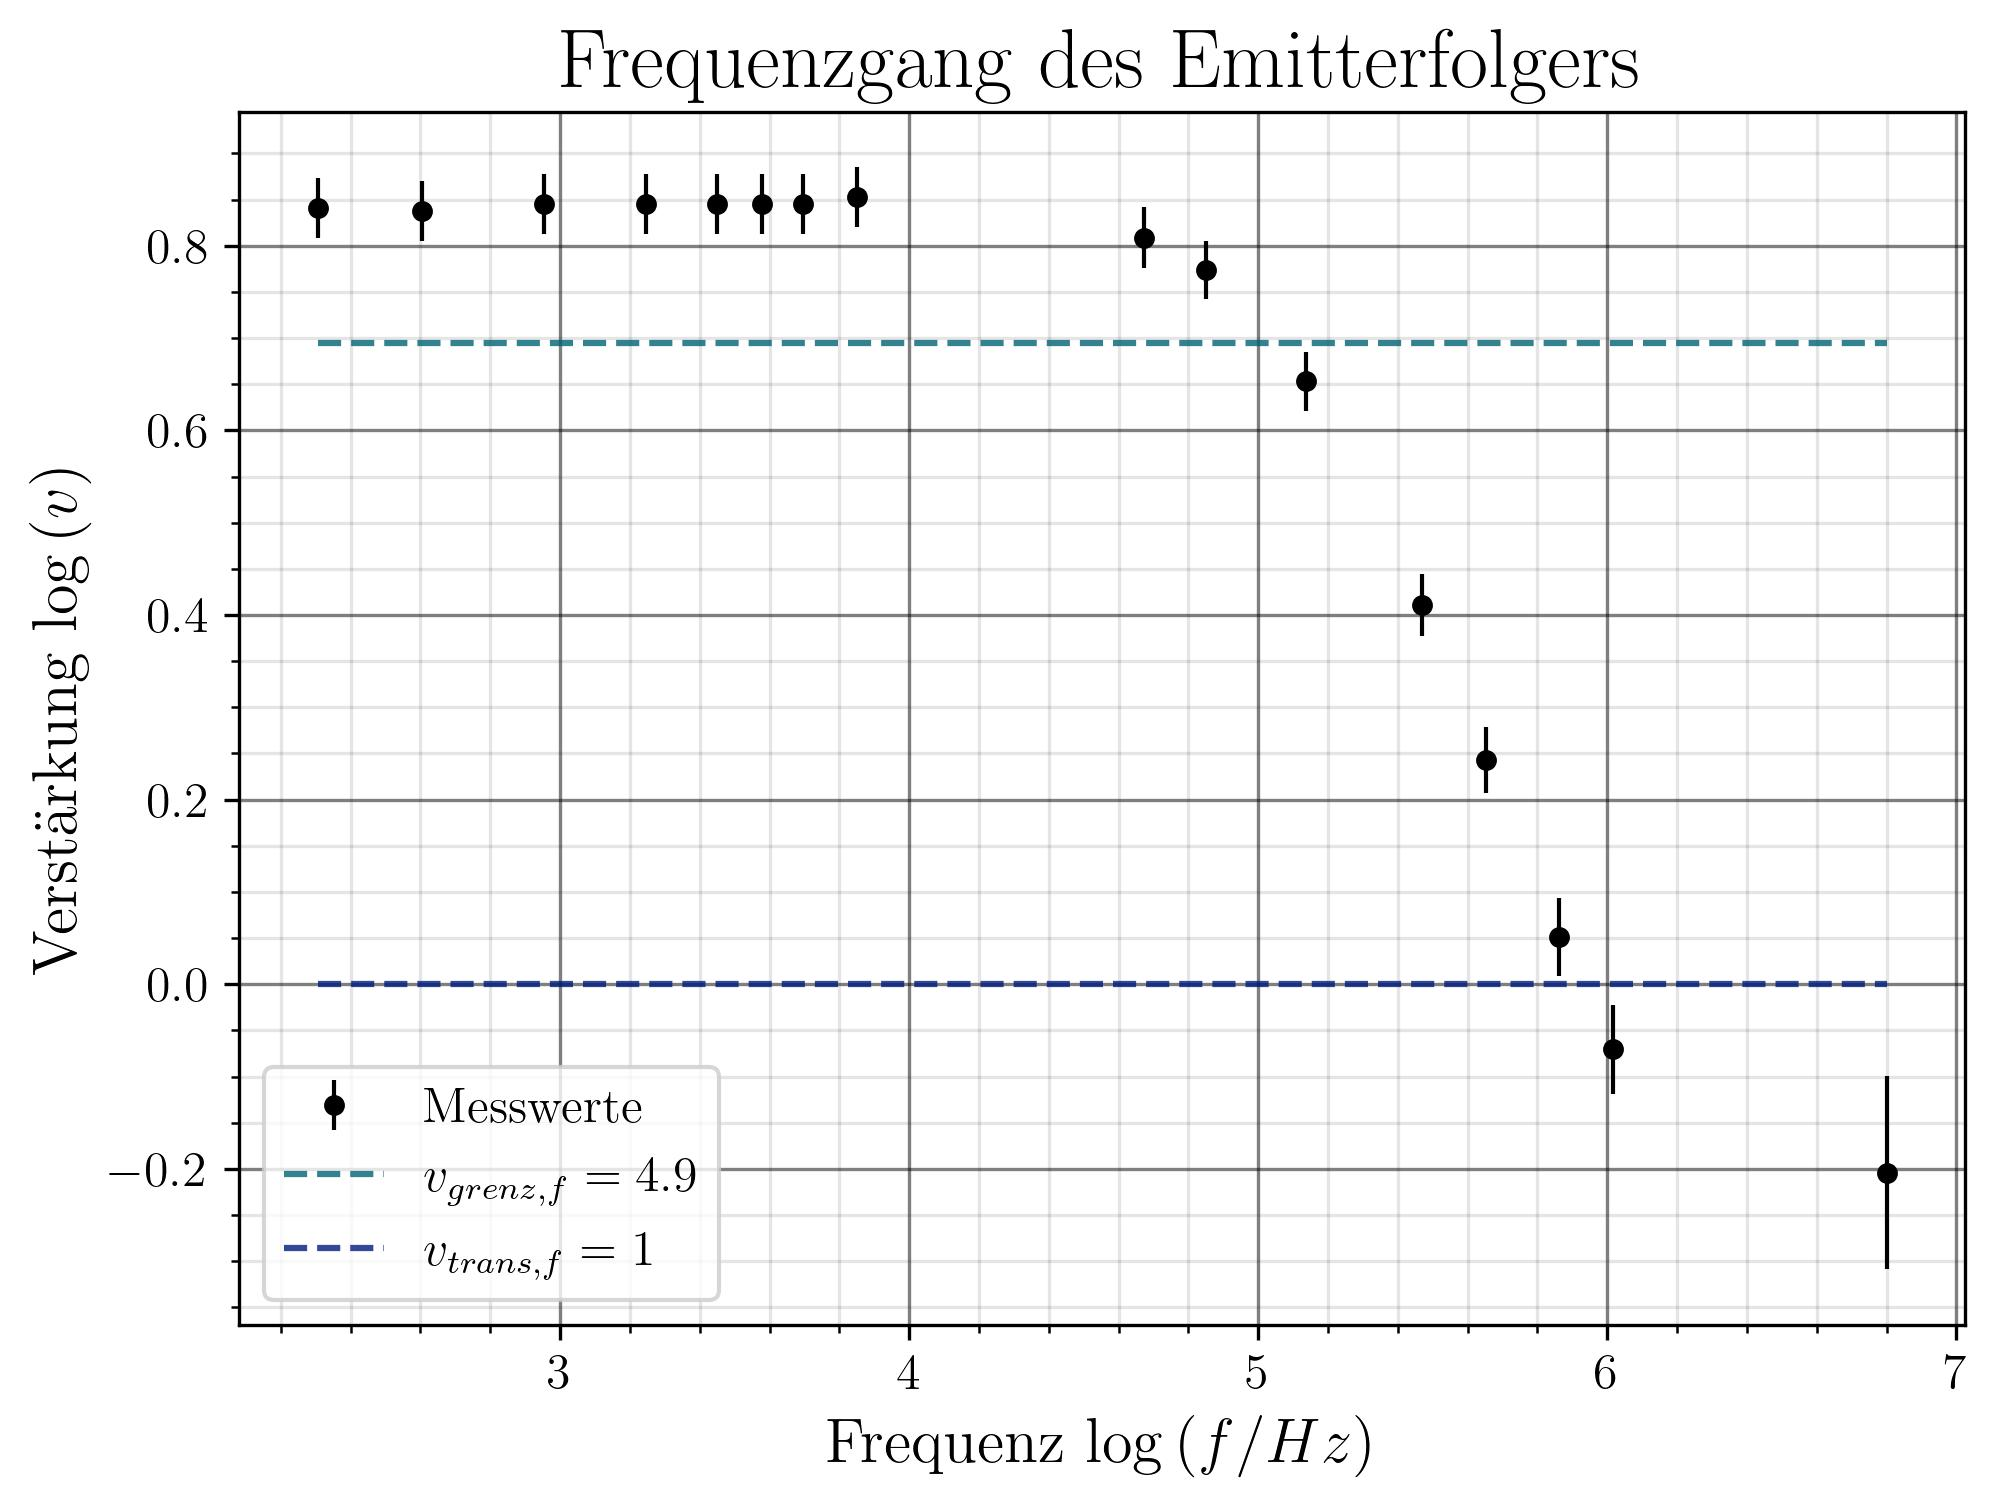
\includegraphics[width=\linewidth]{figs/V4_2e_emitter.jpg}
            \caption{Linke Abbildung}
        \end{subfigure}
        \hspace{1cm}
        \begin{subfigure}{0.4\textwidth}
            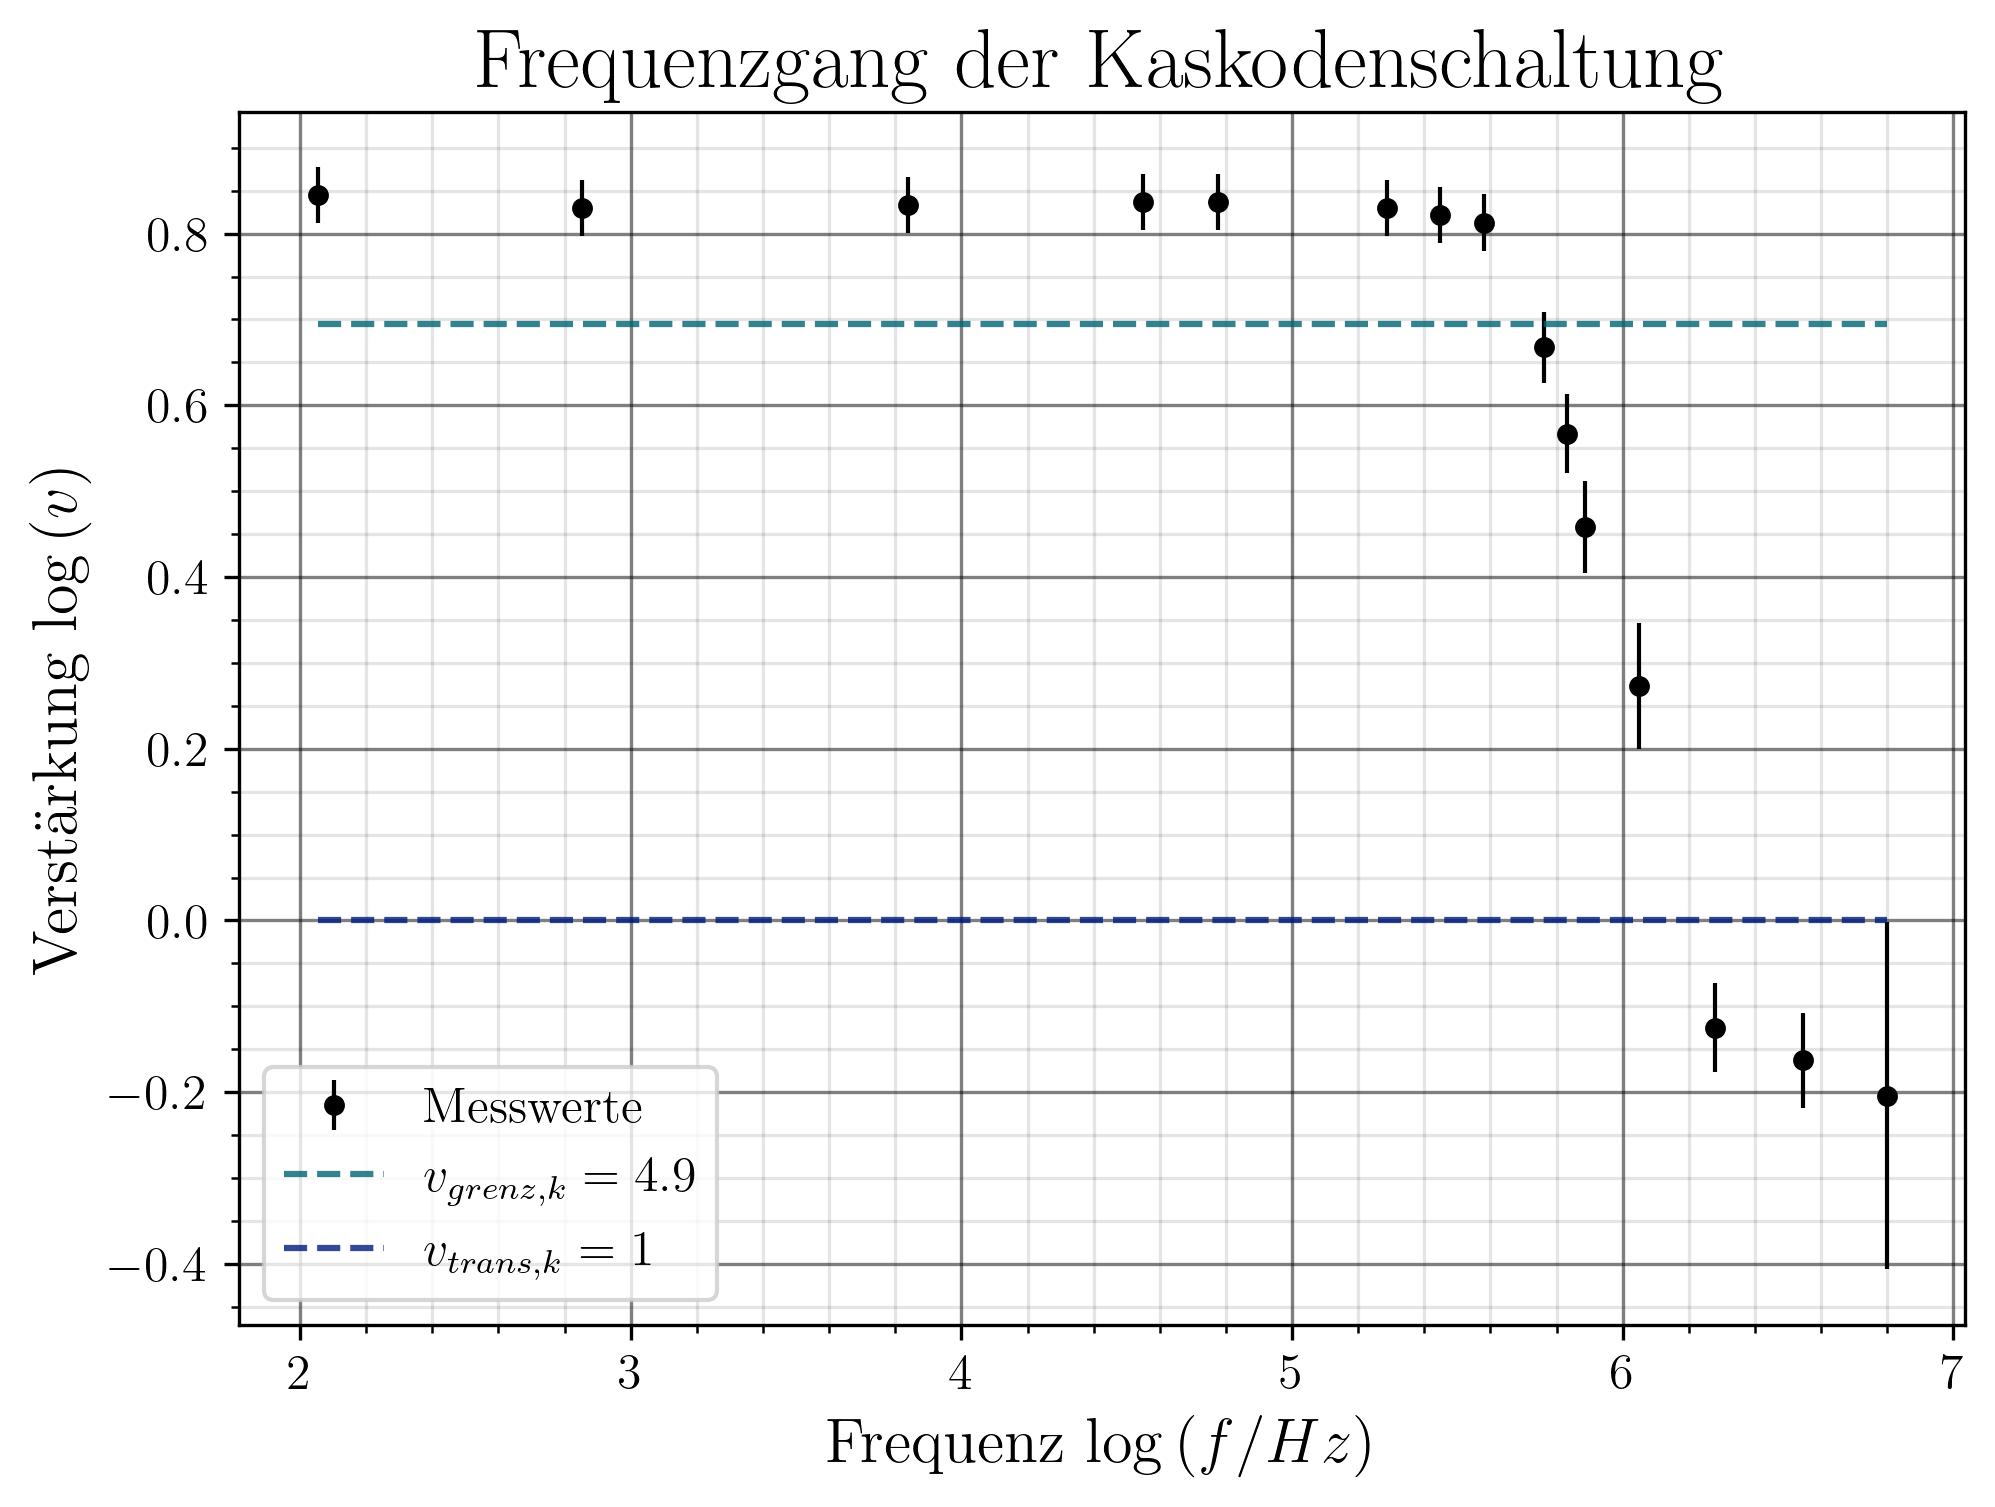
\includegraphics[width=\linewidth]{figs/V4_2e_kaskode.jpg}
            \caption{Rechte Abbildung}
            \label{fig:frequ_kaskode}
        \end{subfigure}
        \caption{Gesamtabbildung}
    \end{figure}

    \begin{figure}[H]
        \centering
        \begin{minipage}{0.4\textwidth}
            \centering
            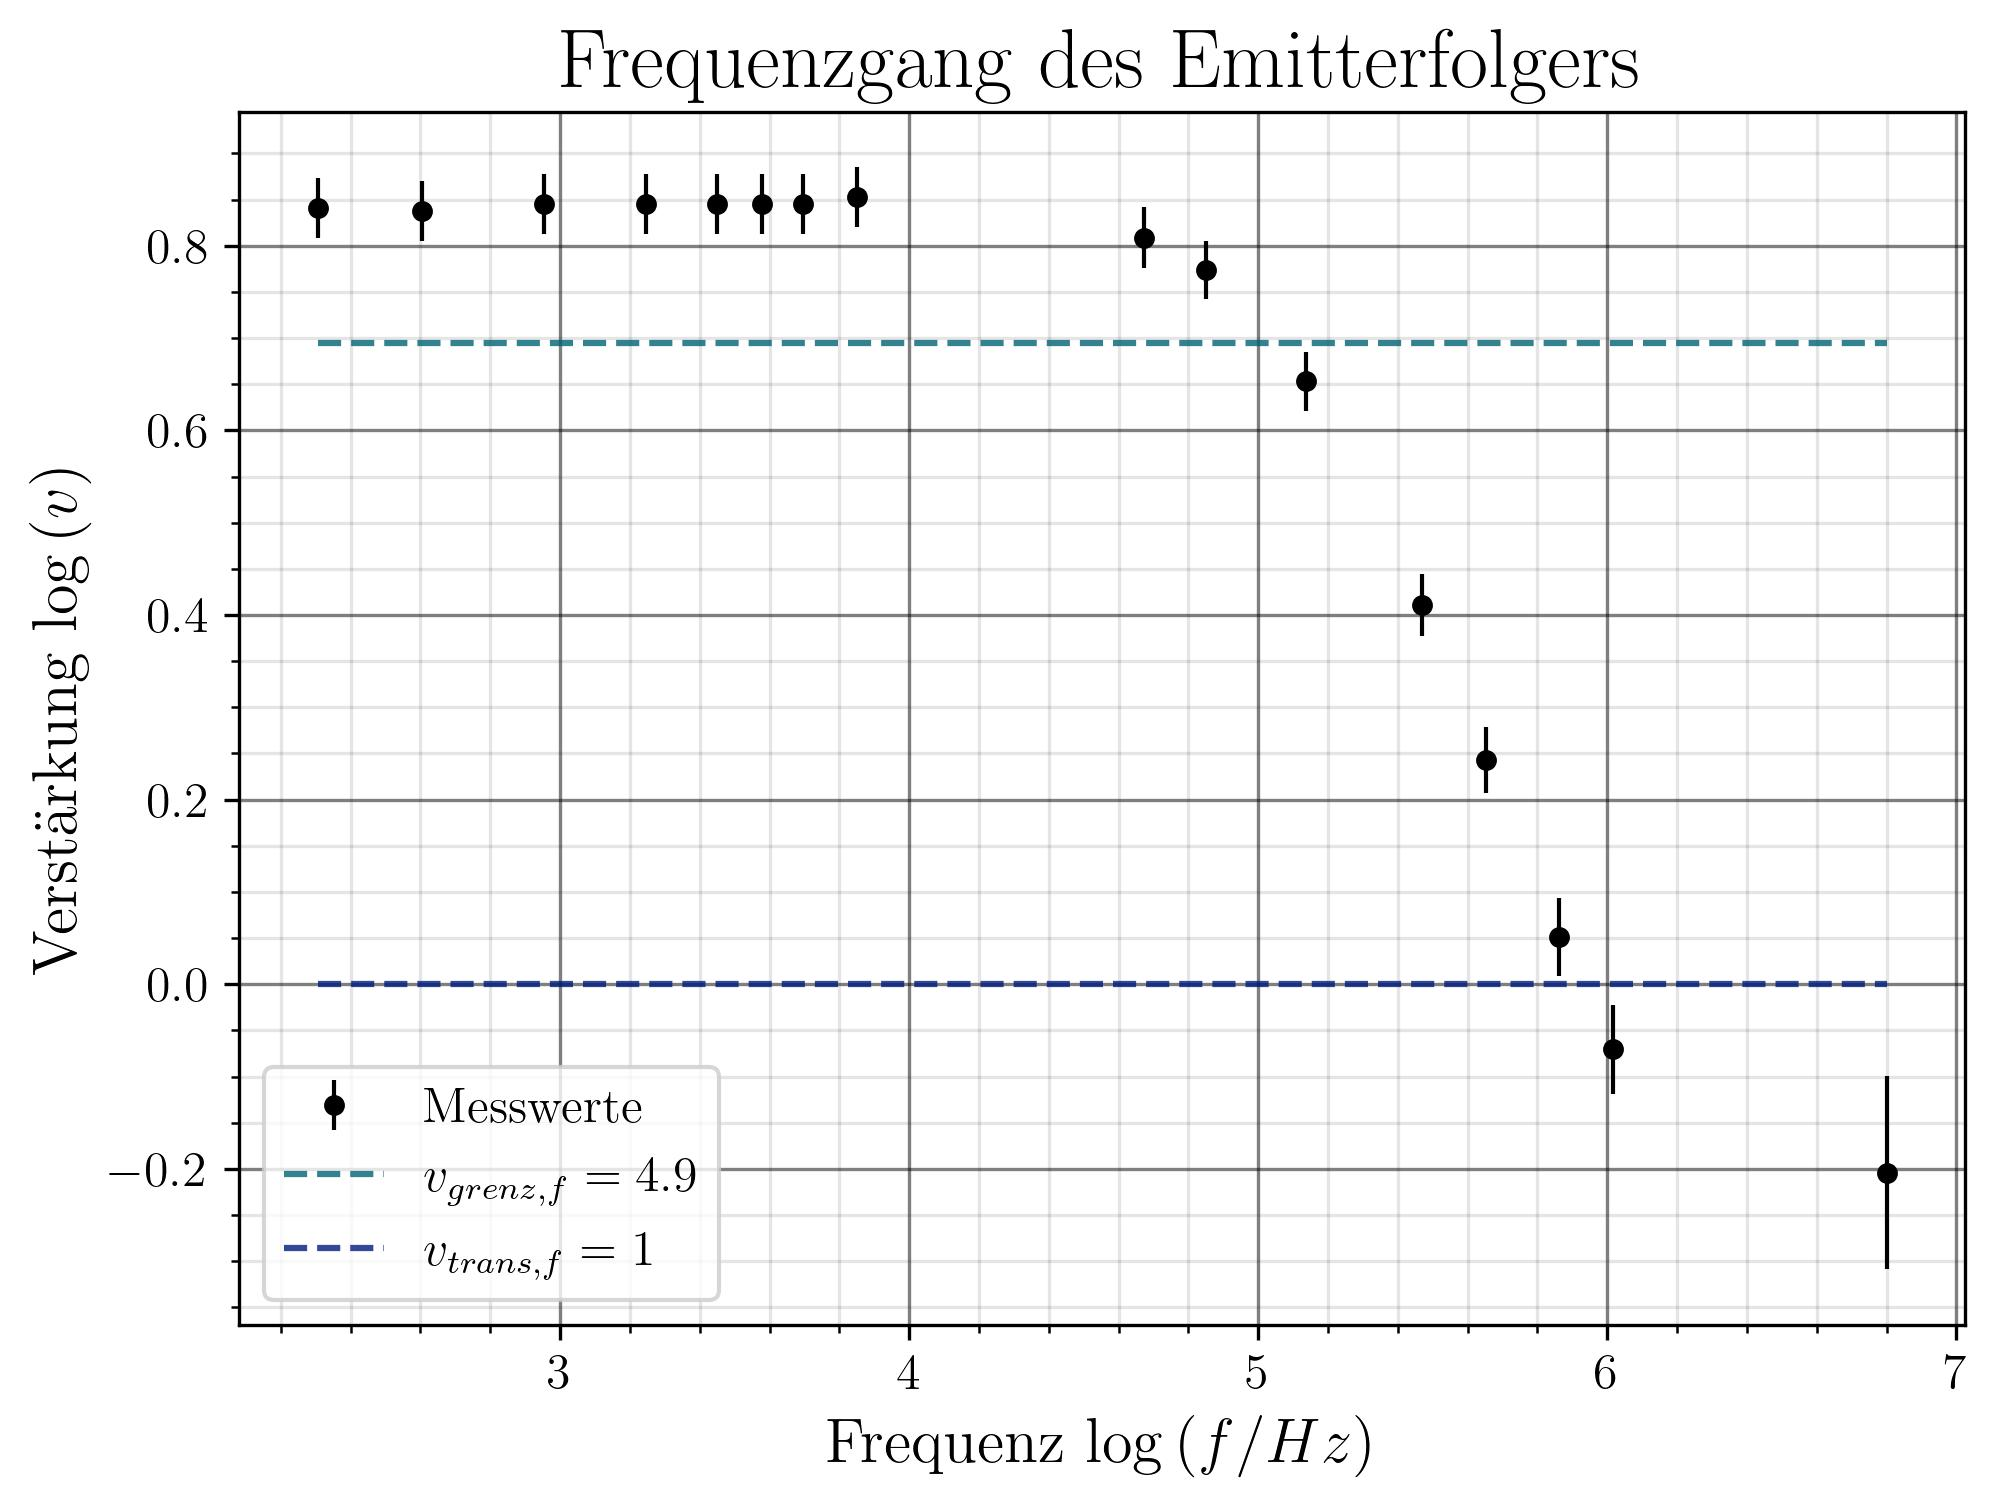
\includegraphics[width=\linewidth]{figs/V4_2e_emitter.jpg}
            \caption{Abbildung neben Text}
        \end{minipage} 
        \hspace{1cm}
        \begin{minipage}{0.4\textwidth}
            Text neben Abbildung... 
        \end{minipage}
    \end{figure}


    \begin{align}
        & f\sub{measured} = \SI{3.0 \pm 0.5}{\mega\hertz} \\
        & f\sub{theory} = \SI{3.6(2)}{\mega\hertz} 
    \end{align}
    
    \printbibliography

\end{document}